%!TEX root = ../Thesis.tex
\section{Selection of Device}
To determine the best device to collect philological information of the subjects. We took into consideration three different kind of devices, Apple Watch Series 2, Garmin Vivoactive VR and BITalino (r)evolution Plugged Kit BT. We decided to go with BITalino after taking into consideration the following factors.
\subsection{Kinds of Physiological Signals}
We required the device to be able to collect Electrocardiogram (ECG) and Electrodermal Activity (EDA) of the subjects. Apple Watch Series 2 and Garmin Vivoactive VR can only collect Heart Rate Variability (HRV) and not a raw Electrocardiogram (ECG). Moreover, the data obtained from these devices are filtered by the manufacturers proprietary filtering algorithms, hence adding an unknown variable. Neither are these devices equipped to collect Electrodermal Activity (EDA) information of subjects. While, BITalino is equipped with both ECG and EDA sensors which collect RAW Electrocardiogram (ECG) and Electrodermal Activity (EDA) information of the subjects.
\subsection{Medical Expertise}
Most medical grade devices require technical expertise and knowledge of anatomy to configure and operate. Moreover, the high-end medical devices are expensive and time consuming to operate. Thus, we decided on to highly versatile and easy to operate framework, BITalino.
\subsection{Cost}
We decided to collect data from multiple subjects at once. See Section. Being able to collect information simultaneously from 5-10 subjects simultaneously required the devices to be cost effective. Thus, we decided to go along with BITalino, since it is affordable and easier to scale.
\subsection{Availability of data}
BITalino provides an Application Programming Interface (API). Using which we designed a custom interface to access and synchronize the data with the start and end time of the movies. The device also allows time synchronization between multiple devices which will be discussed in Section \ref{time_sync}.

\todo{Add details from paper - Performance Comparison of Low-cost Hardware Platforms Targeting Physiological Computing Applications}

\section{Ethical Board Review}
Keeping in mind the privacy of the subjects undergoing the experiment. We made sure we did not collect data in any form or manner with which the subject’s identity can be revealed. We thus pseudo-named the subjects while collecting the data with incremental numbers, example, Person\_1, Person\_2...
\paragraph{}
We also made sure that the audio-visual content shown to the users did not create any long-term psychological effect. To make sure our experiment was within the ethical boundaries, we submitted our research project for review to Ethical Review Board, Department of Computer Sciences, Universität des Saarlandes. The board reviewed our research project and came to a conclusion that there are no ethical concerns against the implementation of the research project.
\paragraph{}
We further took consent from each subject by introducing them to the study procedure and its purpose. The subjects were made aware of the risks and discomforts that may occur during the study and had right to withdraw from the study at any point and time.

\section{Anatomy of BITalino}
\subsection{Design Principles}
BITalino is a 100x65x6mm chip on board device that integrates multiple plug and play sensors to measure bio-electrical and bio-mechanical data. The digital back-end is supported by a control block based on ATmega328P micro-controller, and a communication block that uses a Class II Bluetooth v2.0 module for wireless data transfer to a base station (example. Computer, Mobile Phone etc).\cite{silva_bitalino:_2014}
\paragraph{}
The device is capable of recording at 1, 10, 100 or 1000 Hz frequency. The device has four 10-bit analog ports and two 6-bit analog ports which can be utilized to connect to plug and play sensors to record physiological signals of the subjects. The detailed specification of the device is listed in the table below.
\todo{Add the table with specs}
\todo{Write about data samples / data frames, MAC Address}
\subsection{ECG Sensor}
The ECG sensor of BITalino operates in range of -1.5mV to +1.5mV and bandwidth between 0.5-40Hz. The sensor has gain of 1100 and input impedance of 100GOhms. The ECG Sensor is connected to three-lead electrode, two of which are placed on left and right under the collar bone and one is placed on the right of belly acting as ground. The visualization of the lead placement is shown in the figure \ref{fig:ecg_lead_placement}
\begin{figure}
	\centering
	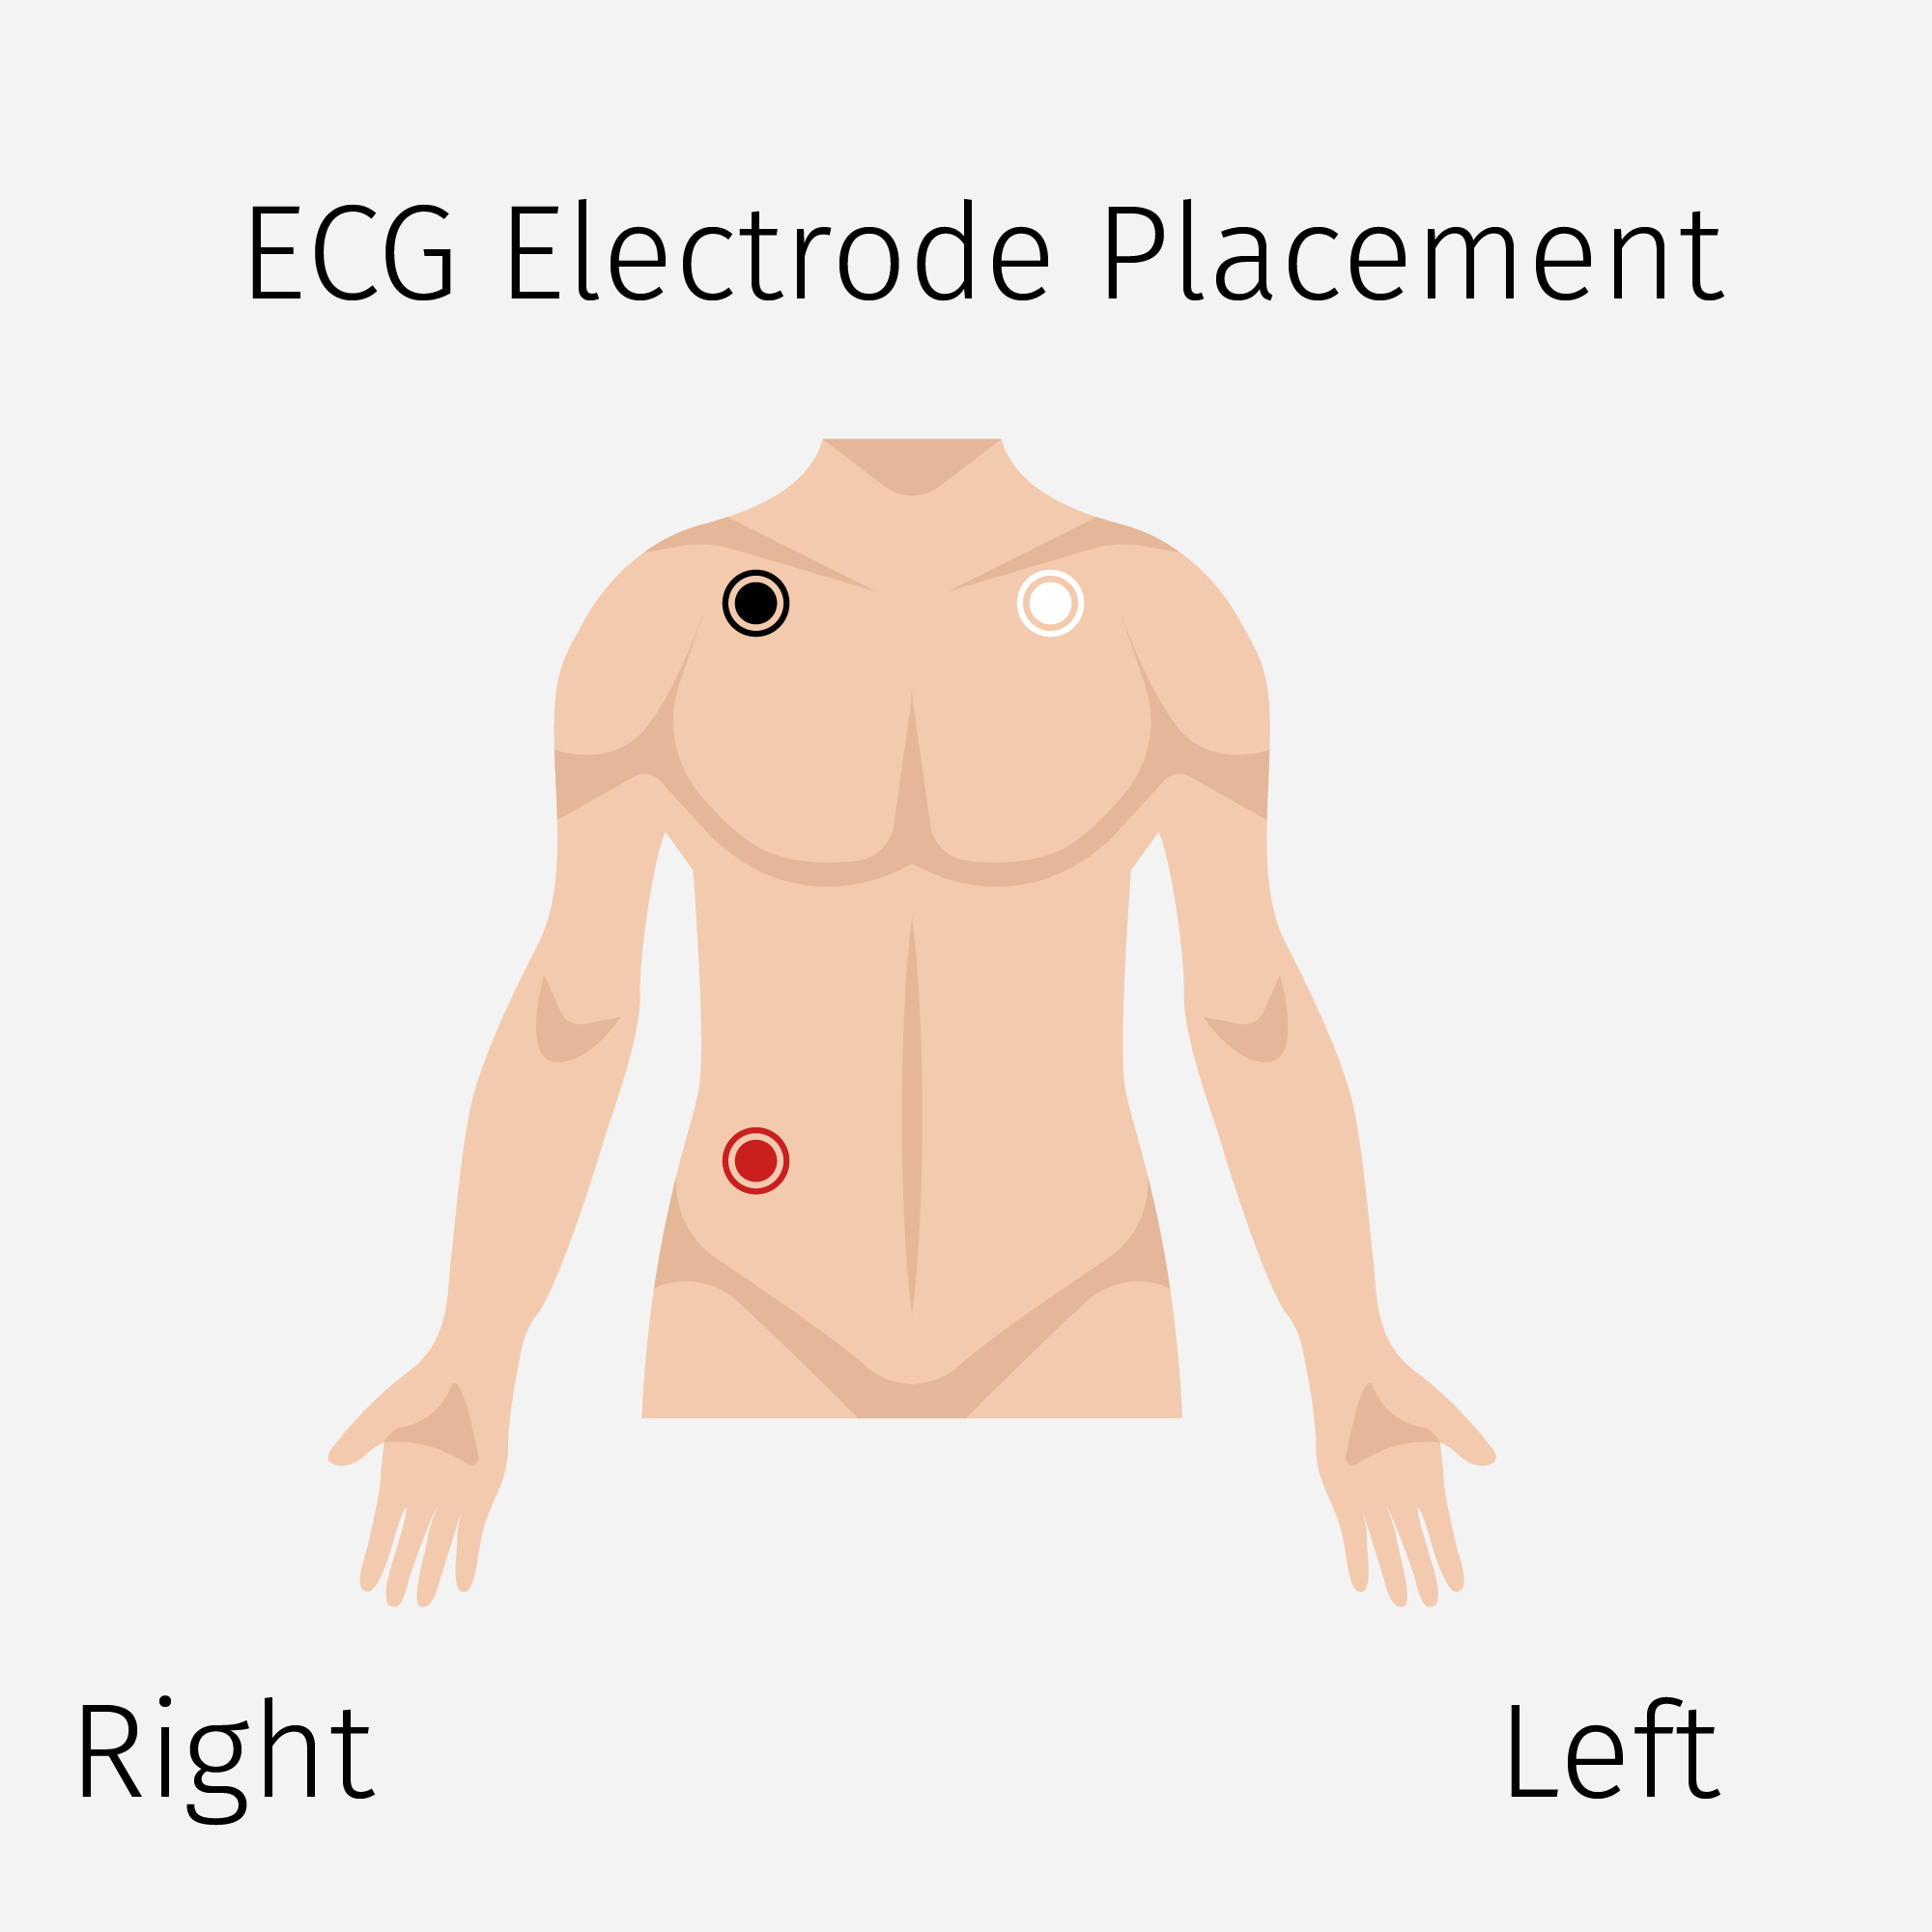
\includegraphics[width=100mm]{ECG.jpg}
	\caption{ECG Lead placement}
	\label{fig:ecg_lead_placement}
\end{figure}
\subsection{EDA Sensor}
The EDA sensor of BITalino operates between 1.8-5.5V with bandwidth between 0-2.8Hz. The EDA sensor is designed to record the EDA in the range between 0-25mueS with input voltage of 3.3V. The EDA sensor is connected to a two-lead electrode which are placed on the tip or center of index and middle finger of the subjects. The visualization of the lead placement is shown in the figure \ref{fig:eda_lead_placement}
\begin{figure}
	\centering
	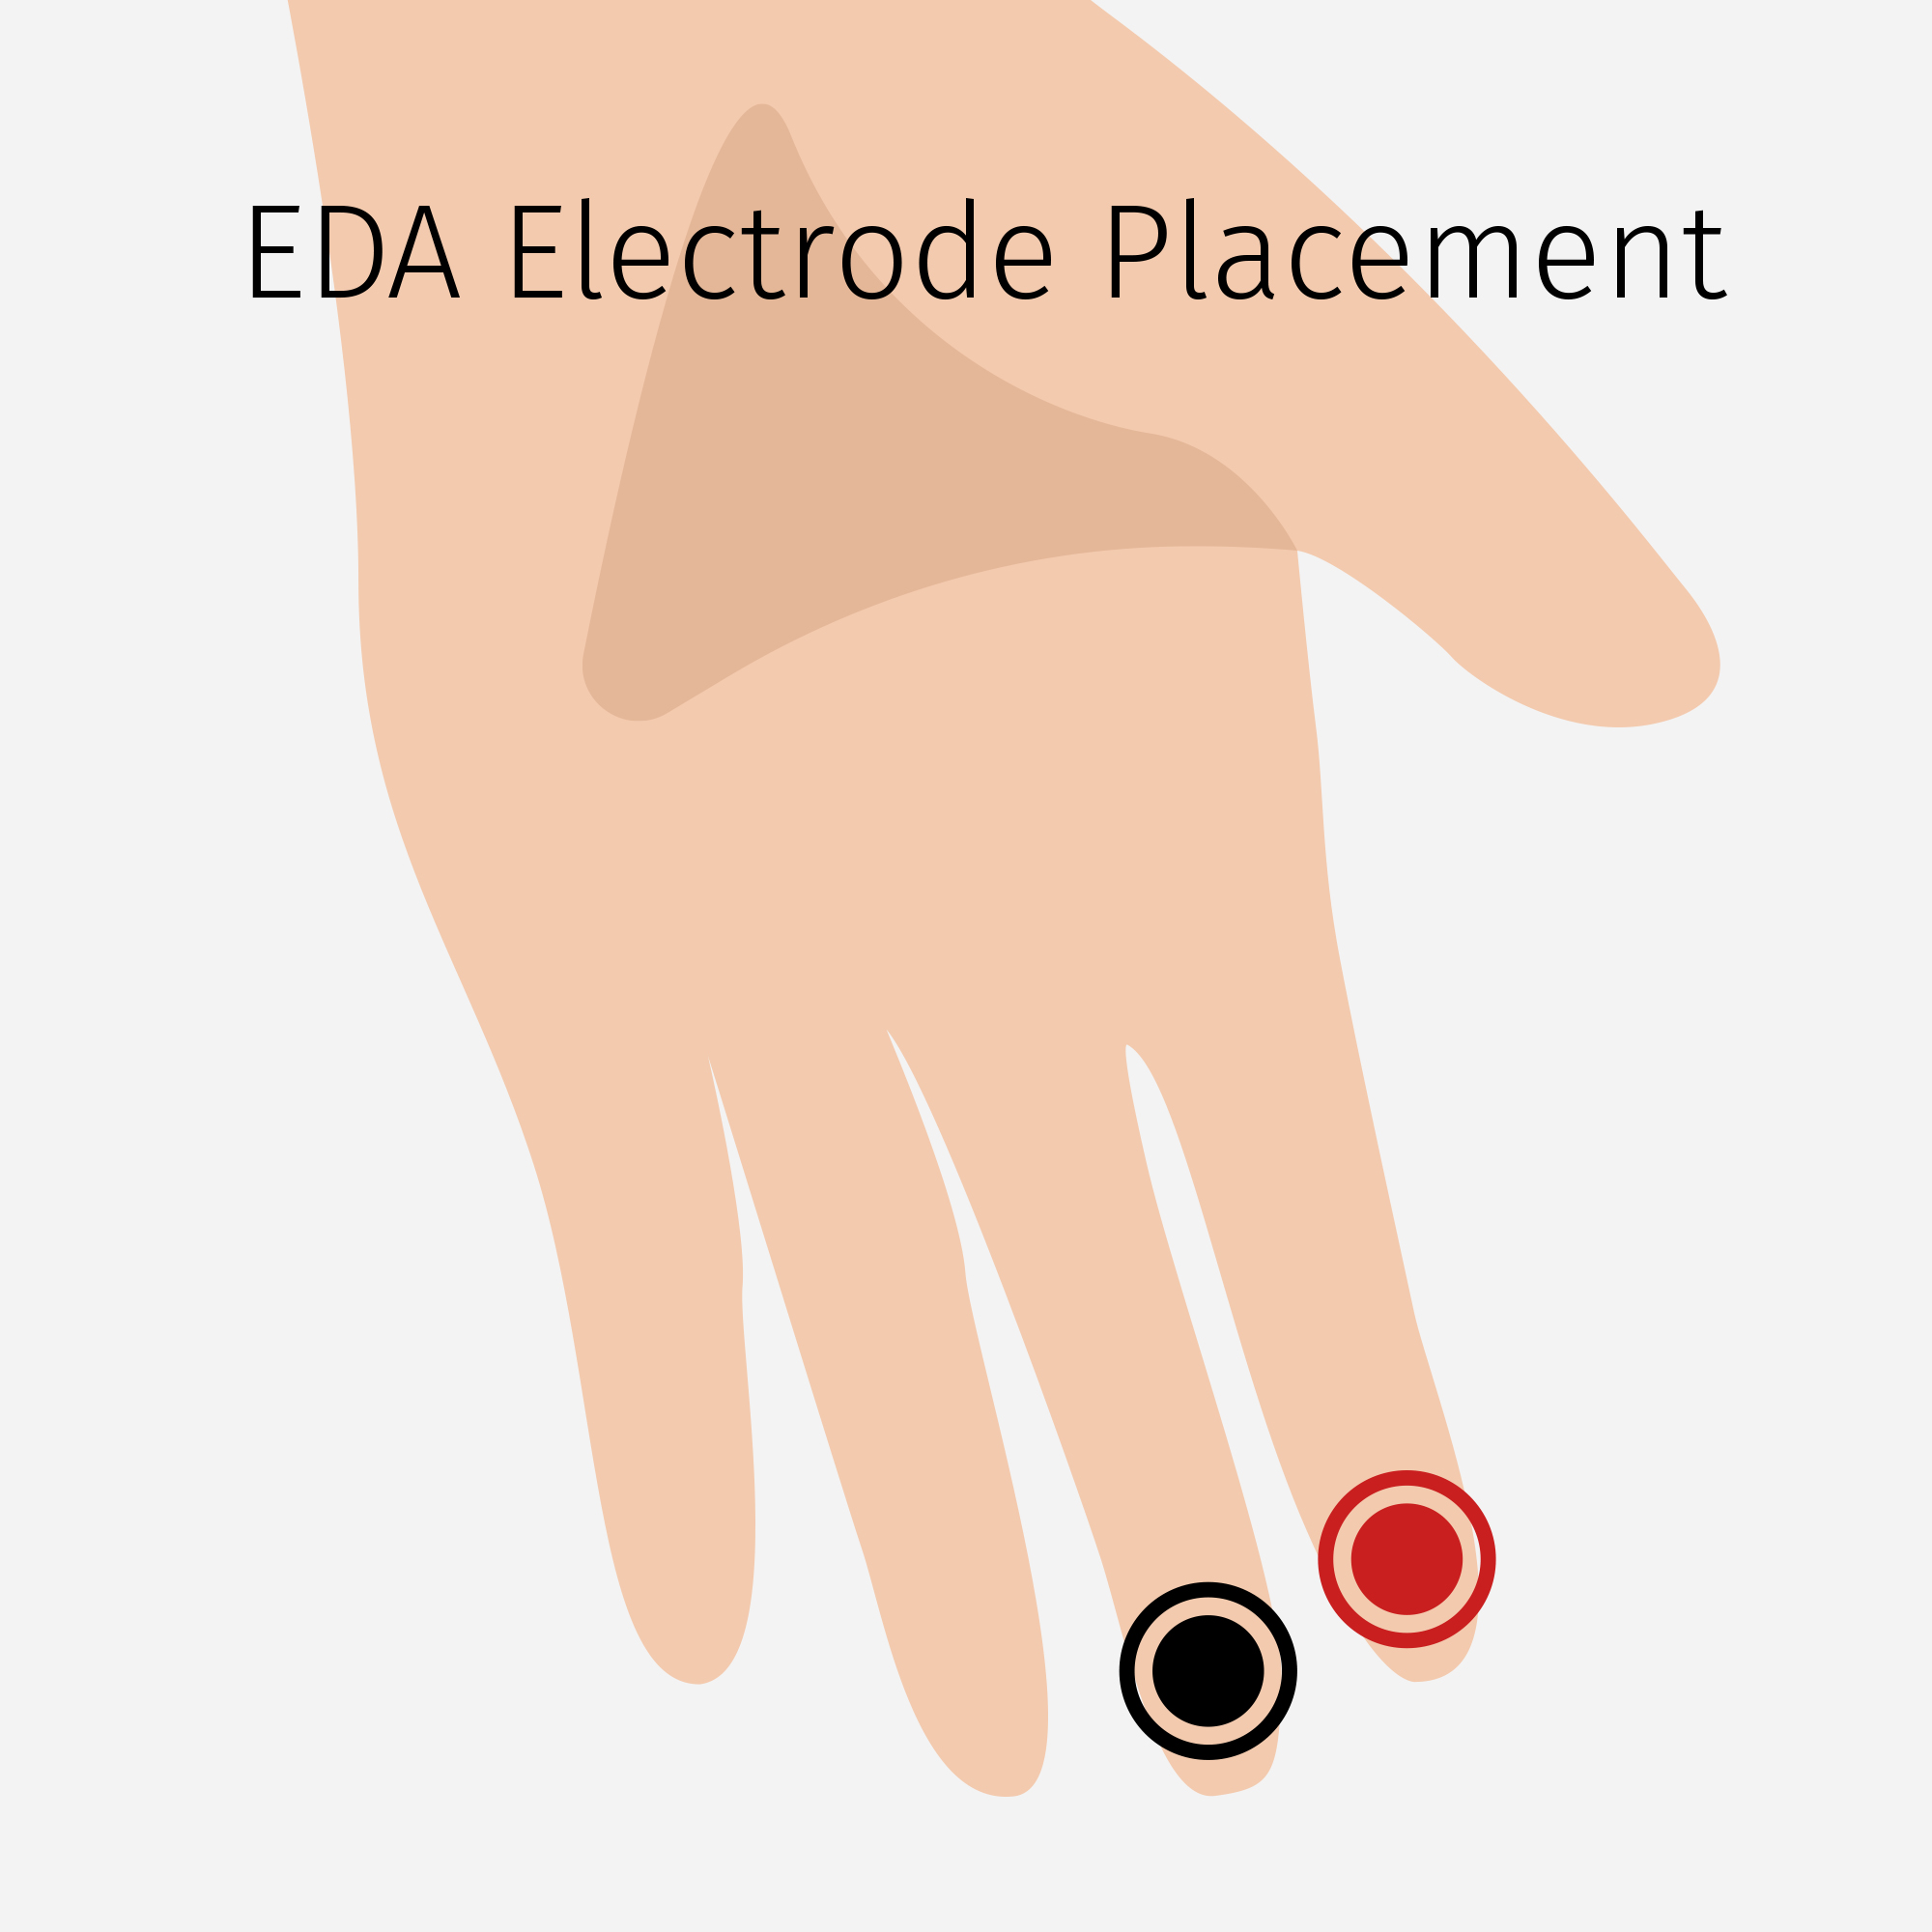
\includegraphics[width=100mm]{EDA.jpg}
	\caption{EDA Lead placement}
	\label{fig:eda_lead_placement}
\end{figure}
\paragraph{}
During our initial test run we realized that the certain subjects EDA was crossing the threshold value when the leads were placed at tip of the finger. Hence, we had to adjust the leads to center of index finger to get proper input.

\section{BITalino Configuration}
We set on to measure Electrocardiogram (ECG) and Electrodermal Activity (EDA) of the subjects. Hence, we took advantage of ECG and EDA sensors of the BITalino. The sensors were then connected to two of four BITalino’s analog ports. The leads of the electrodes were then connected to the subject. Since we wished to collect data from multiple subjects two subjects were connected to one BITalino device. We did not utilize the other two 6-bit analog ports. 
\paragraph{}
To further increase the number of subjects we utilized multiple BITalino devices. Having multiple devices connected and being recorded from posed a challenge of synchronizing the devices. Time synchronization of multiple devices is explained in Section \ref{time_sync}.
\paragraph{}
To make sure that we had the data required in a time synchronized and annotated with the right tags, we custom designed the interface utilizing BITalino API. The details of which are discussed in Section \ref{custom_int}.

\subsection{Time Synchronization}
\label{time_sync}
When multiple devices were connected we noticed that there was a minor delay of about 190ms when the recording began. Since the devices are accessed in a loop and data is recorded serially over the Bluetooth, there was a need to synchronize the devices.
\paragraph{}
We took advantage of input and output digital ports of BITalino. The devices were connected in master and slave configuration where output of master was connected to input on the slave device. Each time the sample is read from the master device, it would trigger the output which in turn will switch the input on the slave device. Thereafter, the data can be synchronized based on the input and output bits.

\subsection{Custom Interface}
\label{custom_int}
The key requirement of our experiment was to accurately determine the start and end time of them movies and correspond them to the data being collected and tag the collected data for analysis. We designed the custom interface in client-server architecture. The server-side interface is showing in the figure \ref{fig:bitalino_cc}
\paragraph{}
The server-side of the interface is designed for device management and playback control of the movies. The interface initiates the connection with BITalino devices. The interface also enables the channels to be tagged with pseudo-names of the subjects which are then written to a file. When the recording is started the server-side program reads the data from devices in a loop and writes it to their respective files.
\paragraph{}
The second feature on server-side enables playback control on the client-side using Websockets. The interface allows for playing and pausing of the movie, each of these actions then create a log file with timestamp of the action performed along with the movie name.
\begin{figure}
	\centering
	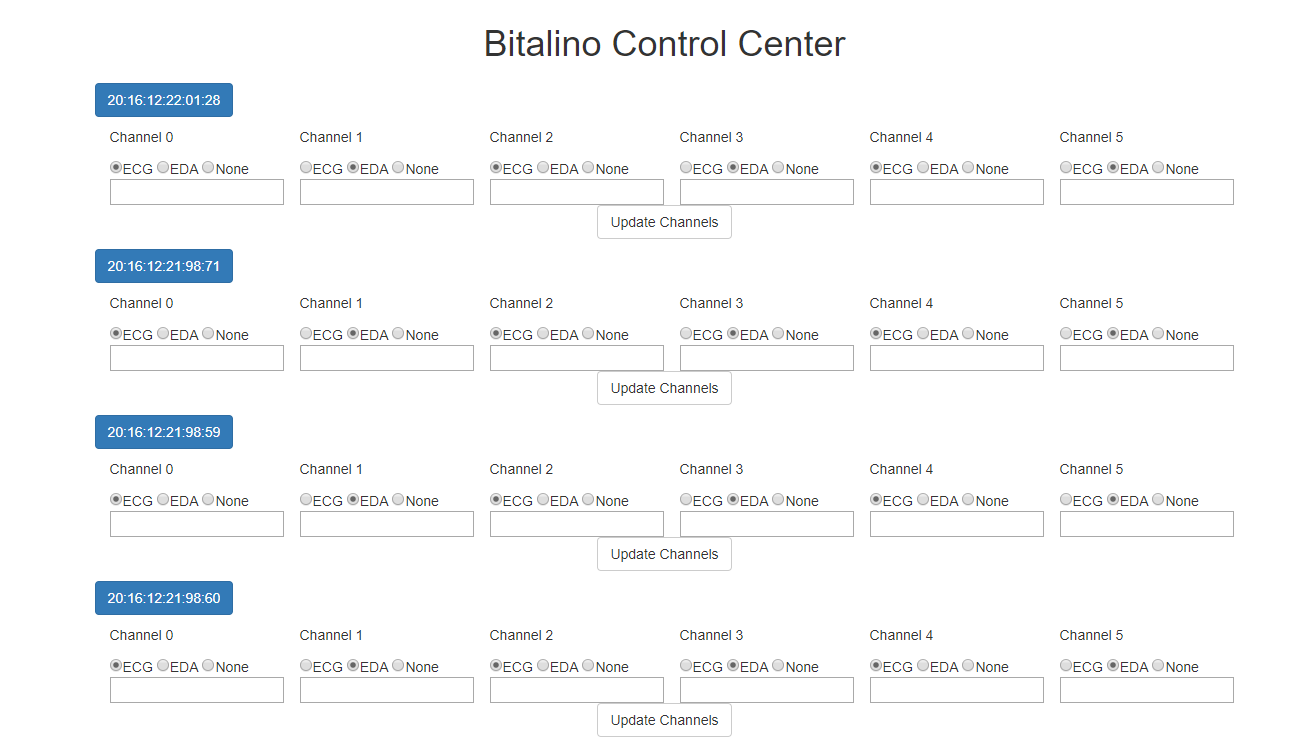
\includegraphics[width=150mm]{bitalino_cc.png}
	\caption{BITalino Control Center}
	\label{fig:bitalino_cc}
\end{figure}

